\documentclass[aspectratio=169,10pt]{beamer}
\newcommand{\TalkShort}{Research roadmap}
% Visual reference: Matteo Di Sante, 13_06_26_slides_soaring_ctrw.tex.
% Steel-blue title bar, Palatino, Pisa seal, white pages and a pale title band.
\usepackage[T1]{fontenc}
\usepackage[utf8]{inputenc}
\usepackage[english]{babel}
\usepackage{mathpazo}
\usefonttheme{serif}
\usepackage{amsmath,amssymb,bm,booktabs,array,graphicx,tikz,microtype}
\usetikzlibrary{arrows.meta,calc,positioning}
\usepackage{siunitx}
\sisetup{group-separator={,},group-minimum-digits=4}
\usepackage{pgfpages}
\ifdefined\Speakernotes
  \setbeameroption{show notes on second screen=right}
\else
  \setbeameroption{hide notes}
\fi
\definecolor{pisablue}{RGB}{74,96,121}
\definecolor{pisablight}{RGB}{192,206,220}
\definecolor{accent}{RGB}{26,118,179}
\definecolor{para}{HTML}{3477A8}
\definecolor{hang}{HTML}{B5482A}
\definecolor{beginner}{HTML}{6A3D9A}
\definecolor{expert}{HTML}{C98A1E}
\definecolor{teal}{HTML}{2E7D8A}
\definecolor{wine}{HTML}{8E3B5C}
\definecolor{muted}{HTML}{666666}
\setbeamercolor{structure}{fg=pisablue}
\setbeamercolor{normal text}{fg=black,bg=white}
\setbeamercolor{frametitle}{fg=white,bg=pisablue}
\setbeamercolor{alerted text}{fg=accent}
\setbeamercolor{block title}{fg=white,bg=pisablue}
\setbeamercolor{block body}{fg=black,bg=pisablight!28}
\setbeamercolor{discussion}{fg=pisablue,bg=pisablight!30}
\setbeamercolor{button}{fg=white,bg=pisablue}
\setbeamerfont{button}{size=\normalsize}
\setbeamersize{text margin left=7mm,text margin right=7mm}
\setbeamertemplate{navigation symbols}{}
\setbeamertemplate{itemize item}{\textcolor{pisablue}{\small$\bullet$}}
\setbeamertemplate{itemize subitem}{\textcolor{pisablue}{\textendash}}
\setbeamertemplate{itemize/enumerate body begin}{\setlength{\itemsep}{0.55em}}
\setbeamertemplate{frametitle}{%
  \nointerlineskip
  \begin{beamercolorbox}[wd=\paperwidth,ht=9mm,dp=3mm,center]{frametitle}
    \large\insertframetitle\strut
  \end{beamercolorbox}
  \begin{tikzpicture}[remember picture,overlay]
    \node[anchor=north east,text=white,inner sep=0pt,xshift=-2.3mm,yshift=-4.2mm]
      at(current page.north east){\small\insertframenumber};
  \end{tikzpicture}
}
\setbeamertemplate{footline}{%
  \hspace{7mm}\textcolor{muted}{\fontsize{6.5}{8}\selectfont
    Matteo Di Sante\enspace|\enspace\TalkShort}\vspace{2mm}
}
\newcommand{\kw}[1]{\textcolor{accent}{#1}}
\newcommand{\source}[1]{\par\vspace{1mm}{\fontsize{7}{8.3}\selectfont\color{muted}#1\par}}
% Discussion prompts belong only on the companion notes page.
\newcommand{\question}[1]{\note{\par\textbf{Discussion.} #1\par\medskip}}
\newcommand{\takeaway}[1]{\par\vfill
  \begin{beamercolorbox}[wd=\linewidth,sep=5pt]{discussion}
    \small #1
  \end{beamercolorbox}}
\newcommand{\fig}[2][54mm]{\includegraphics[width=\linewidth,height=#1,keepaspectratio]{assets/#2}\par}
\newcommand{\speaker}[1]{\note{#1}}
\setbeamertemplate{note page}{%
  \vspace{4mm}\noindent%
  \begin{minipage}{\linewidth}
    {\small\color{pisablue}\TalkShort\quad|\quad Slide \insertframenumber}\par\medskip
    {\normalsize\bfseries\insertframetitle}\par\medskip
    {\small\insertnote}
  \end{minipage}
}
\newcommand{\refitem}[3]{\href{#1}{#2}\hfill {\color{muted}#3}\par\medskip}
\newcommand{\titleframe}[4]{%
\begin{frame}[plain]
\begin{tikzpicture}[remember picture,overlay]
 \fill[pisablue](current page.south west)rectangle(current page.north east);
 \fill[pisablight](current page.south west)rectangle([yshift=20mm]current page.south east);
 \node[text=white,align=center,text width=.92\paperwidth]at(current page.center)
   {{\LARGE\bfseries #1}};
 \node[text=pisablue,align=center]at([yshift=10mm]current page.south)
   {{\normalsize Version: 14/09/2026}\\[2mm]
    {\small #3}};
\end{tikzpicture}
\note{#4}
\end{frame}}
% Marks a thesis subsection boundary: a PDF bookmark plus a full-page divider,
% so each block of slides can be traced back to its exact place in the thesis.
\newcommand{\subsectionframe}[2]{%
\subsection{#2}
\begin{frame}[plain,noframenumbering]
\begin{tikzpicture}[remember picture,overlay]
 \fill[pisablue](current page.south west)rectangle(current page.north east);
 \node[text=pisablight,align=center,text width=.82\paperwidth]
   at([yshift=10mm]current page.center){{\normalsize Thesis~\S#1}};
 \node[text=white,align=center,text width=.82\paperwidth]
   at([yshift=-4mm]current page.center){{\Large\bfseries #2}};
\end{tikzpicture}
\end{frame}}
\newcommand{\backupstart}{%
\appendix
\begin{frame}[plain,noframenumbering]
\begin{tikzpicture}[remember picture,overlay]
 \fill[pisablue](current page.south west)rectangle(current page.north east);
 \node[text=white,align=center]at(current page.center)
  {{\LARGE\bfseries Discussion material}\\[4mm]{\large Extra figures, derivations and references}};
\end{tikzpicture}
\end{frame}}
\hypersetup{colorlinks=true,urlcolor=accent,linkcolor=accent,pdfauthor={Matteo Di Sante}}
% A notes sheet contains a second rendering of the slide. Disable its duplicate
% destinations; the normal slide PDF retains all hyperlinks and the viewer button.
\ifdefined\Speakernotes\hypersetup{draft}\fi

\usepackage{xfp}
% Generated by measure_cadence.py from the 16 Sep 2026 coverage tables.
\newcommand{\CadParaOne}{70.7}
\newcommand{\CadParaTwo}{7.8}
\newcommand{\CadParaFive}{17.0}
\newcommand{\CadParaSlow}{4.6}
\newcommand{\CadParaLost}{29.3}
\newcommand{\CadParaLostFlights}{30.1}
\newcommand{\CadParaUpToTen}{99.2}
\newcommand{\CadParaLabelled}{69.9}
\newcommand{\CadParaHours}{480,383}
\newcommand{\CadHangOne}{29.2}
\newcommand{\CadHangTwo}{12.9}
\newcommand{\CadHangFive}{40.2}
\newcommand{\CadHangSlow}{17.7}
\newcommand{\CadHangLost}{70.8}
\newcommand{\CadHangLostFlights}{72.0}
\newcommand{\CadHangUpToTen}{99.5}
\newcommand{\CadHangLabelled}{29.1}
\newcommand{\CadHangHours}{20,372}

% Generated by render_glide_autocorrelation.py from glide-autocorrelation.csv.
\newcommand{\GlideCohortGlides}{50}
\newcommand{\GlideMaxLag}{49}
\newcommand{\GlideFitA}{0.63}
\newcommand{\GlideFitXi}{26}
\newcommand{\GlideFitLo}{1}
\newcommand{\GlideFitHi}{33}
\newcommand{\GlideOpenFlights}{963}
\newcommand{\GlideOpenOne}{0.71}
\newcommand{\GlideOpenLast}{0.16}
\newcommand{\GlideOpenMin}{0.16}
\newcommand{\GlideOpenMinLag}{49}
\newcommand{\GlideClosedFlights}{2,407}
\newcommand{\GlideClosedOne}{0.65}
\newcommand{\GlideClosedLast}{0.00}
\newcommand{\GlideClosedMin}{$-$0.27}
\newcommand{\GlideClosedMinLag}{26}
\newcommand{\GlideClosedZero}{13}

% Generated by scripts/tesi/ch02_dataset/generate_pipeline_census.py -- do not edit.
\newcommand{\StatPipeParaAttempted}{186052}
\newcommand{\StatPipeParaKept}{156406}
\newcommand{\StatPipeParaKeptPct}{84.1}
\newcommand{\StatPipeParaBaroWitnessPct}{72.1}
\newcommand{\StatPipeParaDropPipelineRaised}{0}
\newcommand{\StatPipeParaDropFewerThanTwoFixes}{27}
\newcommand{\StatPipeParaDropNoUsableAltitudeChannel}{697}
\newcommand{\StatPipeParaDropNoSustainedFlight}{197}
\newcommand{\StatPipeParaDropCleaningRebuiltTooMuch}{550}
\newcommand{\StatPipeParaDropDurationBelowMinimum}{2084}
\newcommand{\StatPipeParaDropDurationAboveMaximum}{3}
\newcommand{\StatPipeParaDropPathBelowMinimum}{173}
\newcommand{\StatPipeParaDropAltitudeRangeBelowMinimum}{4899}
\newcommand{\StatPipeParaDropMeanGroundSpeedAboveTheFixLevelBound}{0}
\newcommand{\StatPipeParaDropExtentOutOfReachOfTheFirstFix}{217}
\newcommand{\StatPipeParaDropNoNativeCadence}{0}
\newcommand{\StatPipeParaDropNoSegmentSurvived}{20798}
\newcommand{\StatPipeParaDropShorterThanSmoothingWindow}{1}
\newcommand{\StatPipeParaMedianDurationMin}{158}
\newcommand{\StatPipeParaMedianPathKm}{89}
\newcommand{\StatPipeParaMedianDtS}{1}
\newcommand{\StatPipeParaSplitPct}{9.9}
\newcommand{\StatPipeParaMedianSegments}{1}
\newcommand{\StatPipeParaInterpPct}{0.58}
\newcommand{\StatPipeParaTrimmedPct}{1.32}
\newcommand{\StatPipeParaRemovedPct}{1.83}
\newcommand{\StatPipeParaAltInvalidPct}{0.056}
\newcommand{\StatPipeParaFlaggedKeptPct}{0.68}
\newcommand{\StatPipeParaFrozenFlightsPct}{31.3}
\newcommand{\StatPipeParaBoundariedFlightsPct}{0.12}
\newcommand{\StatPipeParaBoundariedTotal}{1688}
\newcommand{\StatPipeParaInSegmentSteps}{1369613762}
\newcommand{\StatPipeHangAttempted}{6716}
\newcommand{\StatPipeHangKept}{6094}
\newcommand{\StatPipeHangKeptPct}{90.7}
\newcommand{\StatPipeHangBaroWitnessPct}{84.7}
\newcommand{\StatPipeHangDropPipelineRaised}{0}
\newcommand{\StatPipeHangDropFewerThanTwoFixes}{0}
\newcommand{\StatPipeHangDropNoUsableAltitudeChannel}{135}
\newcommand{\StatPipeHangDropNoSustainedFlight}{1}
\newcommand{\StatPipeHangDropCleaningRebuiltTooMuch}{53}
\newcommand{\StatPipeHangDropDurationBelowMinimum}{79}
\newcommand{\StatPipeHangDropDurationAboveMaximum}{0}
\newcommand{\StatPipeHangDropPathBelowMinimum}{1}
\newcommand{\StatPipeHangDropAltitudeRangeBelowMinimum}{155}
\newcommand{\StatPipeHangDropMeanGroundSpeedAboveTheFixLevelBound}{0}
\newcommand{\StatPipeHangDropExtentOutOfReachOfTheFirstFix}{5}
\newcommand{\StatPipeHangDropNoNativeCadence}{0}
\newcommand{\StatPipeHangDropNoSegmentSurvived}{193}
\newcommand{\StatPipeHangDropShorterThanSmoothingWindow}{0}
\newcommand{\StatPipeHangMedianDurationMin}{184}
\newcommand{\StatPipeHangMedianPathKm}{163}
\newcommand{\StatPipeHangMedianDtS}{3}
\newcommand{\StatPipeHangSplitPct}{20.5}
\newcommand{\StatPipeHangMedianSegments}{1}
\newcommand{\StatPipeHangInterpPct}{0.30}
\newcommand{\StatPipeHangTrimmedPct}{0.84}
\newcommand{\StatPipeHangRemovedPct}{0.72}
\newcommand{\StatPipeHangAltInvalidPct}{0.036}
\newcommand{\StatPipeHangFlaggedKeptPct}{0.96}
\newcommand{\StatPipeHangFrozenFlightsPct}{65.4}
\newcommand{\StatPipeHangBoundariedFlightsPct}{0.21}
\newcommand{\StatPipeHangBoundariedTotal}{408}
\newcommand{\StatPipeHangInSegmentSteps}{34559873}
\newcommand{\PipeCensusTable}{%
\begin{tabular}{|l|r|r|}
\hline
\textbf{Why the flight was dropped} & paragliders & hang gliders \\
\hline
unreadable track & 27 & 0 \\
no usable GNSS altitude & 697 & 135 \\
never airborne & 197 & 1 \\
integrity gate & 550 & 53 \\
shorter than the duration cut & 2{,}084 & 79 \\
longer than the duration cut & 3 & 0 \\
path below the floor & 173 & 1 \\
altitude activity below the floor & 4{,}899 & 155 \\
out of reach of its own first fix & 217 & 5 \\
no segment survived resampling & 20{,}798 & 193 \\
no segment carries the smoothing window & 1 & 0 \\
\hline
\textbf{retained} & \textbf{156{,}406} (84.1\%) & \textbf{6{,}094} (90.7\%) \\
\hline
\end{tabular}}

\hypersetup{pdftitle={From flight logs to optimal paths},pdfsubject={Internship and thesis roadmap, October 2026 -- February 2027}}
\setbeamertemplate{frametitle}{}
\setbeamertemplate{footline}{}
\setbeamerfont{note page}{size=\small}
% Narrow boxes: break between words, never inside them.
\hyphenpenalty=10000
\exhyphenpenalty=10000

% Flight phases, in the hues of Vilpellet et al., Fig. 3 (blue, red, green).
\definecolor{glide}{HTML}{1F4FBF}
\definecolor{search}{HTML}{C8262B}
\definecolor{climb}{HTML}{11823B}
\definecolor{wait}{HTML}{8A6240}
\definecolor{rising}{HTML}{D9480F}
% Individual flights in the solo/group sketches (Okabe--Ito).
\definecolor{flA}{HTML}{0072B2}
\definecolor{flB}{HTML}{009E73}
\definecolor{flC}{HTML}{CC79A7}
\definecolor{flD}{HTML}{E69F00}
% Plan view of thermalling: #1 x, #2 y, #3 colour, #4 radius, #5 turns; loops drift east by .5 mm per turn.
\newcommand{\loops}[5]{\draw[#3,line width=.75pt,domain=0:#5*360,samples=50*#5,smooth]plot({#1-#4+#4*cos(\x)+.5*\x/360},{#2+#4*sin(\x)});}
% One colour per step, reused on every slide and in the timeline.
\definecolor{sOne}{HTML}{7A8794}
\definecolor{sTwo}{HTML}{1A76B3}
\definecolor{sThree}{HTML}{2E7D8A}
\definecolor{sFour}{HTML}{3F4A9C}
\definecolor{sFive}{HTML}{C98A1E}
\definecolor{sSix}{HTML}{B5482A}
\definecolor{sTool}{HTML}{6A3D9A}

% Page coordinates in mm from the top-left corner, y downwards (160 x 90).
\newcommand{\txt}[5][]{\node[anchor=north west,inner sep=0pt,text width=#4mm,align=flush left,font=\fontsize{10}{12}\selectfont,#1]at(#2,#3){#5};}
\newcommand{\smalltxt}[5][]{\txt[font=\fontsize{8.5}{10.5}\selectfont,#1]{#2}{#3}{#4}{#5}}
\newcommand{\bulitem}[1]{\noindent\makebox[3mm][l]{\textcolor{pisablue}{\textbullet}}\parbox[t]{\dimexpr\linewidth-3mm}{\raggedright #1}\par\vspace{1.2mm}}
\newcommand{\badge}[4][3.2]{\fill[#2,draw=white,line width=.6pt](#3)circle(#1);\node[text=white,font=\bfseries\fontsize{8.5}{9}\selectfont]at(#3){#4};}
% Title bar. #1 step colour (or pisablue), #2 step number (empty: none), #3 title, #4 tag.
\newcommand{\startslide}[4]{%
 \begin{tikzpicture}[remember picture,overlay,shift={(current page.north west)},x=1mm,y=-1mm]
 \fill[white](0,0)rectangle(160,90);
 \fill[pisablue](0,0)rectangle(160,12.5);
 \if\relax\detokenize{#2}\relax
  \node[anchor=west,inner sep=0pt,text=white,font=\fontsize{15}{17}\selectfont\bfseries]at(7,6.4){#3};
 \else
  \badge[3.6]{#1}{11,6.4}{\fontsize{10}{10}\selectfont#2}
  \node[anchor=west,inner sep=0pt,text=white,font=\fontsize{15}{17}\selectfont\bfseries]at(17.5,6.4){#3};
 \fi
 \node[anchor=east,inner sep=0pt,text=pisablight,font=\fontsize{8.5}{10}\selectfont]at(148,6.6){#4};
 \node[anchor=east,inner sep=0pt,text=white,font=\fontsize{8}{9}\selectfont]at(155,6.6){\insertframenumber};}
\newcommand{\finishslide}{\end{tikzpicture}}
\newcommand{\bottomline}[1]{\fill[pisablight!33](7,74.7)rectangle(153,83);
 \node[anchor=west,inner sep=0pt,text width=142mm,align=left,text=pisablue,font=\bfseries\boldmath\fontsize{10}{12}\selectfont]at(10,78.85){#1};}
\newcommand{\credit}[1]{\node[anchor=west,inner sep=0pt,text width=122mm,align=left,text=muted,font=\fontsize{6}{7}\selectfont]at(7,86.5){#1};}
% A rounded card: #1 x, #2 y, #3 width, #4 height, #5 colour, #6 extra style.
\newcommand{\card}[6][]{\draw[rounded corners=1.5mm,fill=#6!8,draw=#6!70,line width=.8pt,#1](#2,#3)rectangle++(#4,#5);}
\newcommand{\arrowto}[5][]{\draw[-{Latex[length=2.2mm]},line width=1pt,#2,#1](#3)--(#4)#5;}
% Status marks of the characterisation slide.
\newcommand{\stDone}[1]{\fill[sThree](#1)circle(1.3);}
\newcommand{\stFirst}[1]{\draw[sThree,line width=.6pt](#1)circle(1.3);\fill[sThree](#1)++(0,-1.3)arc(-90:90:1.3)--cycle;}
\newcommand{\stOpen}[1]{\draw[sThree,line width=.6pt](#1)circle(1.3);}

\begin{document}

% 1 ---------------------------------------------------------------------
\begin{frame}[plain]
\begin{tikzpicture}[remember picture,overlay,shift={(current page.north west)},x=1mm,y=-1mm]
 \fill[white](0,0)rectangle(160,90);
 \fill[pisablue](0,0)rectangle(80,72);
 \txt[text=pisablight,font=\bfseries\fontsize{8.5}{10}\selectfont]{9}{11}{60}{\textls[80]{INTERNSHIP \& THESIS ROADMAP}}
 \txt[text=white,font=\bfseries\fontsize{21}{25}\selectfont]{9}{19}{70}{From flight logs\\to optimal paths}
 \txt[text=white!85!pisablue,font=\fontsize{11.5}{14.5}\selectfont]{9}{44}{66}{Possible research paths\\and timeline}
 \txt[text=white,font=\fontsize{11}{13}\selectfont]{9}{58}{60}{Matteo Di Sante}
 \txt[text=pisablight,font=\fontsize{8.5}{10}\selectfont]{9}{63.5}{60}{September 2026 -- February 2027}
 \node[anchor=center,inner sep=0pt]at(120,36){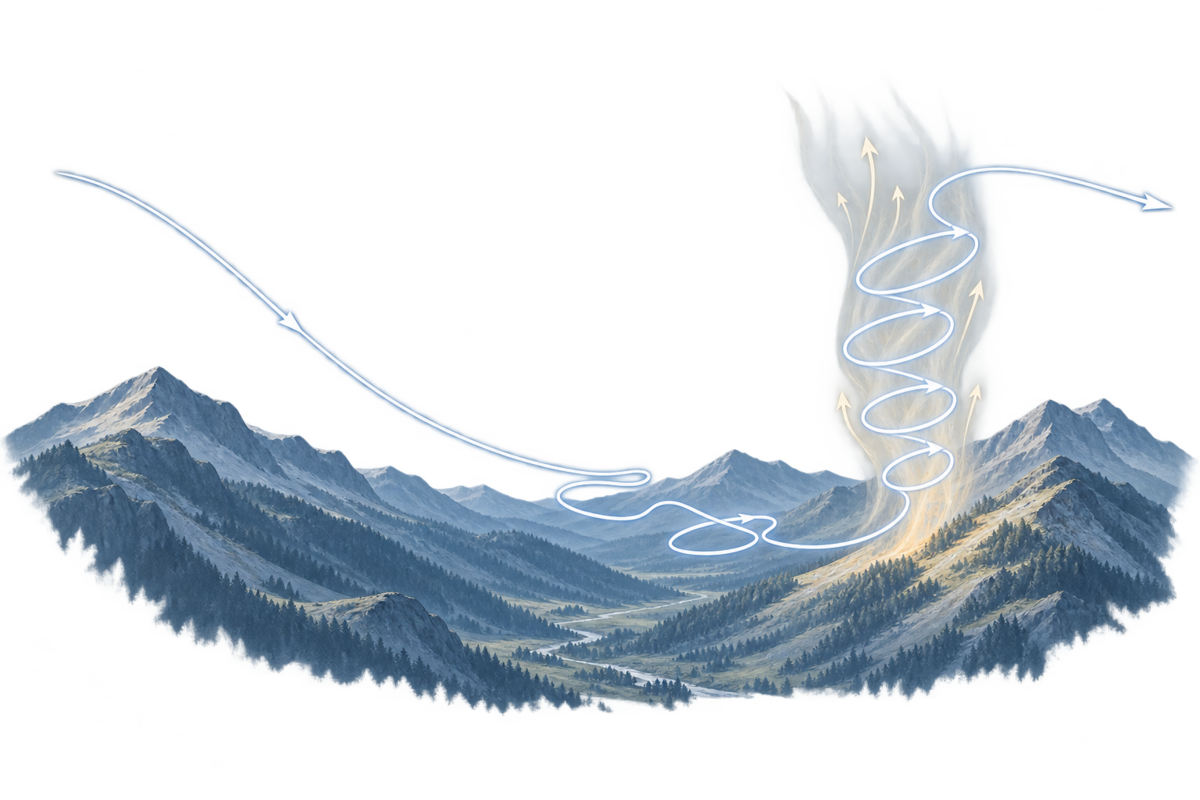
\includegraphics[width=76mm]{assets/cover-flight.png}};
 \draw[pisablight,line width=.6pt](0,72)--(160,72);
 \node[anchor=west,inner sep=0pt]at(9,81.5){
\includegraphics[width=40mm]{assets/econophysics-lab.png}};
 \node[inner sep=0pt]at(82,81.5){
\includegraphics[width=25mm]{assets/cfm.png}};
 \node[anchor=east,inner sep=0pt]at(151,81.5){
\includegraphics[width=37mm]{assets/ilb.pdf}};
\end{tikzpicture}
\speaker{Today: the possible paths for the rest of the internship and the thesis, from October 2026 to February 2027. Six steps. The first is done. Steps 2 and 3 are the foundation. Steps 4, 5 and 6 are research directions built on top of it. A graphical tool is developed in parallel throughout. Cover: AI-generated illustration of a glide, a search and a climb in a thermal.}
\end{frame}

% 2 ---------------------------------------------------------------------
\begin{frame}[plain]
\startslide{pisablue}{}{The plan at a glance}{12 Oct 2026 -- 28 Feb 2027}
 % Day 0 = 12 Oct 2026; 140 days to 1 Mar 2027 over 106 mm.
 \begin{scope}[shift={(46,0)},x=.757mm]
  \fill[muted!12](73,17.5)rectangle(84,71);
  \node[text=muted,font=\fontsize{7}{8}\selectfont]at(78.5,15.8){break};
  \foreach \d in {20,50,81,112}{\draw[muted!40,line width=.4pt](\d,17.5)--(\d,71);}
  \draw[muted!60,line width=.4pt](0,17.5)--(140,17.5);
  \foreach \m/\c in {Oct/10,Nov/35,Dec/65.5,Jan/96.5,Feb/126}{\node[text=muted,font=\bfseries\fontsize{8}{9}\selectfont]at(\c,15.8){\m};}
  % Step 1 is already done.
  \fill[sOne,rounded corners=.8mm](0,19.5)rectangle(14,24.1);
  \node[text=white,font=\bfseries\fontsize{7}{8}\selectfont]at(7,21.8){2 wk};
  \node[anchor=west,inner sep=0pt,font=\fontsize{7.3}{8.5}\selectfont]at(15.3,21.8){\textcolor{sOne!90!black}{\textbf{done \checkmark}}};
  % Foundation and first two directions.
  \foreach \a/\b/\y/\c/\w/\d in {0/14/26/sTwo/2 wk/{continuous-variable HMM},14/35/32.5/sThree/3 wk/{stochastic fingerprints},35/50/39/sFour/2 wk/{glide + wait, angular memory},49/73/45.5/sFive/3 wk/{}}{
   \fill[\c,rounded corners=.8mm](\a,\y)rectangle(\b,\y+4.6);
   \node[text=white,font=\bfseries\fontsize{7}{8}\selectfont]at({(\a+\b)/2},\y+2.3){\w};
   \node[anchor=west,inner sep=0pt,text=\c!80!black,font=\fontsize{7.3}{8.5}\selectfont]at(\b+1.3,\y+2.3){\d};}
  % Step 6 is exploratory: dashed and light.
  \draw[sSix,fill=sSix!22,dashed,line width=.8pt,rounded corners=.8mm](84,52)rectangle(119,56.6);
  \node[text=sSix!80!black,font=\bfseries\fontsize{7}{8}\selectfont]at(101.5,54.3){5 wk};
  \node[anchor=east,inner sep=0pt,text=sSix!80!black,font=\fontsize{7.3}{8.5}\selectfont]at(82.7,54.3){exploratory};
  % Buffer and the parallel tool.
  \fill[muted!70,rounded corners=.8mm](119,58.5)rectangle(140,63.1);
  \node[text=white,font=\bfseries\fontsize{7}{8}\selectfont]at(129.5,60.8){3 wk};
  \fill[sTool,rounded corners=.8mm](0,65.5)rectangle(140,70.1);
  \node[text=white,font=\bfseries\fontsize{7}{8}\selectfont]at(70,67.8){in parallel: its own repository, runs on any PC};
  % Groups.
  \node[anchor=east,inner sep=0pt,text=muted,font=\bfseries\fontsize{6.8}{8}\selectfont]at(140,31.55){\textls[60]{}};
  \node[anchor=east,inner sep=0pt,text=muted,font=\bfseries\fontsize{6.8}{8}\selectfont]at(140,47.8){\textls[60]{}};
 \end{scope}
 \foreach \y/\c/\n/\t/\d in {19.5/sOne/1/Data/{done; simplify 12--25 Oct},26/sTwo/2/Segmentation/12--25 Oct,32.5/sThree/3/Characterisation/26 Oct -- 15 Nov,39/sFour/4/Stochastic model/16--30 Nov,45.5/sFive/5/Solo vs group/30 Nov -- 23 Dec,52/sSix/6/Optimal path/4 Jan -- 7 Feb}{
  \badge[2.4]{\c}{9.5,\y+2.3}{\fontsize{7}{8}\selectfont\n}
  \node[anchor=west,inner sep=0pt,font=\bfseries\fontsize{8.5}{10}\selectfont]at(13.5,\y+1.1){\t};
  \node[anchor=west,inner sep=0pt,text=muted,font=\fontsize{6.5}{7.5}\selectfont]at(13.5,\y+4){\d};}
 \node[anchor=west,inner sep=0pt,font=\bfseries\fontsize{8.5}{10}\selectfont]at(13.5,59.6){Buffer};
 \node[anchor=west,inner sep=0pt,text=muted,font=\fontsize{6.5}{7.5}\selectfont]at(13.5,62.5){7--28 Feb};
 \node[anchor=west,inner sep=0pt,text=sTool!80!black,font=\bfseries\fontsize{8.5}{10}\selectfont]at(13.5,67.8){Graphical tool};
 \bottomline{Buffer: absorb delays, or go deeper on the most interesting results}
\speaker{Six steps. Step 1, data download and preprocessing, is done. Today's preprocessing has too many parameters, is too complex and discards too many flights; I will simplify it in parallel with segmentation, 12--25 October. Segmentation (step 2) and the stochastic characterisation (step 3) are the foundation: the phase labels and the measurement toolbox used by everything that follows. Then three research directions: a stochastic model (step 4), solo versus group flight (step 5), and an exploratory optimal-path study (step 6, dashed because its scope is still open).\par\medskip
Indicative windows: segmentation 12--25 October (2 weeks), characterisation 26 October -- 15 November (3 weeks), stochastic model 16--30 November (2 weeks), solo vs group 30 November -- 23 December (3 weeks), winter break 24 December -- 3 January, optimal path 4 January -- 7 February 2027 (5 weeks), then three weeks of buffer until 28 February. The buffer absorbs delays, or is spent on whatever turns out most interesting: parts of the solo vs group study, of the stochastic model, or of the optimal path. The graphical tool runs in parallel for the whole period. Bars are drawn to scale in calendar days.}
\finishslide\end{frame}

% 3 ---------------------------------------------------------------------
\begin{frame}[plain]
\startslide{sOne}{1}{Data download and preprocessing}{done \checkmark\ \textperiodcentered{} simplify 12--25 Oct}
 % Pipeline: archive -> clean archive.
 \card{7}{18}{64}{38}{sOne}
 \txt[text=pisablue,font=\bfseries\fontsize{11}{13}\selectfont]{11}{21}{56}{Download}
 \txt[text=para,font=\bfseries\fontsize{17}{20}\selectfont]{11}{29}{56}{\num{\StatPipeParaAttempted}}
 \smalltxt{11}{36}{56}{paraglider tracklogs}
 \txt[text=hang,font=\bfseries\fontsize{17}{20}\selectfont]{11}{42}{56}{\num{\StatPipeHangAttempted}}
 \smalltxt{11}{49}{56}{hang-glider tracklogs}
 \arrowto{sOne}{73,37}{87,37}{}
 \node[text=sOne!90!black,font=\fontsize{7.5}{9}\selectfont]at(80,34.6){preprocessing};
 \card{89}{18}{64}{38}{sOne}
 \txt[text=pisablue,font=\bfseries\fontsize{11}{13}\selectfont]{93}{21}{56}{Clean archive}
 \txt[text=para,font=\bfseries\fontsize{17}{20}\selectfont]{93}{29}{56}{\num{\StatPipeParaKept}}
 \smalltxt{93}{36}{56}{paraglider flights (\StatPipeParaKeptPct\%)}
 \txt[text=hang,font=\bfseries\fontsize{17}{20}\selectfont]{93}{42}{56}{\num{\StatPipeHangKept}}
 \smalltxt{93}{49}{56}{hang-glider flights (\StatPipeHangKeptPct\%)}
 % The only open item, set apart.
 \draw[rounded corners=1.8mm,fill=pisablue!9,draw=pisablue,line width=1.3pt](7,59)rectangle(153,83);
 \node[anchor=west,inner xsep=2.6mm,inner ysep=1.6mm,rounded corners=1mm,fill=pisablue,text=white,font=\bfseries\fontsize{10}{11}\selectfont]at(12,71){NEXT};
 \txt[text=pisablue,font=\bfseries\fontsize{14}{16}\selectfont]{34}{61.8}{116}{Simplify the preprocessing}
 \txt[font=\fontsize{10}{12}\selectfont]{34}{68.6}{116}{Today's version has too many parameters, is too complex and discards too many flights (paragliders: \fpeval{round(100-\StatPipeParaKeptPct)}\%).\\ In parallel with segmentation, 12--25 Oct.}
\speaker{The FFVL distance-contest archive is downloaded: 186,052 paraglider and 6,716 hang-glider tracklogs. The preprocessing pipeline cleans the recorded flight, selects flights and projects them to local coordinates, puts them on a uniform time grid and smooths them with a Savitzky--Golay filter. It keeps 156,406 paraglider flights (84.1\%) and 6,094 hang-glider flights (90.7\%). It works, but it has too many parameters, it is too complex, and it discards too many flights for no good reason: today paragliders lose \fpeval{round(100-\StatPipeParaKeptPct)}\% of the downloaded tracklogs. I will simplify it in parallel with the segmentation work, 12--25 October.}
\finishslide\end{frame}



% 5 ---------------------------------------------------------------------
\begin{frame}[plain]
\startslide{sTwo}{2}{Segmentation: from 1\,Hz to any logger}{12--25 Oct \textperiodcentered{} 2 weeks}
 % Three cards: what exists, why it is not enough, what comes next.
 \card{7}{17}{46}{53}{muted}
 \card{57}{17}{46}{53}{sSix}
 \card{107}{17}{46}{53}{sTwo}
 \fill[sSix](53.6,40)--(56.4,43.5)--(53.6,47)--cycle;
 \fill[sTwo](103.6,40)--(106.4,43.5)--(103.6,47)--cycle;
 % 1. Vilpellet's HMM.
 \txt[text=muted!80!black,font=\bfseries\fontsize{12}{14}\selectfont]{11}{20}{40}{Vilpellet's HMM}
 \foreach \l/\y in {{$X^{v_z}$: climbing?}/29,{$X^{\mathrm{curv}}$: turning one way?}/36,{$X^{\mathrm{str}}$: straight?}/43}{
  \node[anchor=west,inner xsep=1.6mm,inner ysep=1.2mm,rounded corners=1.1mm,fill=white,draw=muted!70,line width=.5pt,font=\bfseries\fontsize{9}{10}\selectfont]at(11,\y){\l};}
 \smalltxt[text=muted,font=\fontsize{8.5}{10}\selectfont]{11}{48.5}{40}{yes/no, on a rolling 30\,s window}
 \smalltxt[font=\bfseries\fontsize{10}{12}\selectfont]{11}{57}{40}{Checked in the viewer: works well, but misses some climbs}
 % 2. Only 1 Hz.
 \txt[text=sSix!80!black,font=\bfseries\fontsize{12}{14}\selectfont]{61}{20}{40}{Only for 1\,Hz}
 \begin{scope}[shift={(72,0)}]
  \def\s{.4}% mm per second, 30 s window over 12 mm inside 70 s
  \foreach \y in {28.2,33.4}{\draw[muted,line width=.4pt](0,\y+1.6)--(70*\s,\y+1.6);}
  \foreach \t in {0,...,70}{\draw[glide!70,line width=.22pt](\t*\s,28.6)--(\t*\s,30.6);}
  \foreach \t in {0,5,...,70}{\fill[glide](\t*\s,35)circle(.42);}
  \foreach \y in {28.2,33.4}{\fill[sTwo,fill opacity=.18](20*\s,\y)rectangle(50*\s,\y+3.2);\draw[sTwo,line width=.5pt](20*\s,\y)rectangle(50*\s,\y+3.2);}
 \end{scope}
 \smalltxt[font=\bfseries\fontsize{8}{9}\selectfont]{61}{28.4}{11}{1\,Hz}
 \smalltxt[font=\bfseries\fontsize{8}{9}\selectfont]{61}{33.6}{11}{5\,s}
 \txt[text=para,font=\bfseries\fontsize{19}{21}\selectfont]{61}{41}{20}{\fpeval{round(\CadParaLostFlights)}\%}
 \txt[text=hang,font=\bfseries\fontsize{19}{21}\selectfont]{83}{41}{20}{\fpeval{round(\CadHangLostFlights)}\%}
 \smalltxt[font=\fontsize{8}{9.5}\selectfont]{61.3}{48.6}{20}{paragliders}
 \smalltxt[font=\fontsize{8}{9.5}\selectfont]{83.3}{48.6}{20}{hang gliders}
 \smalltxt[font=\bfseries\fontsize{10}{12}\selectfont]{61}{57}{40}{of flights left out: loggers slower than 1\,Hz}
 % 3. Next.
 \txt[text=sTwo!80!black,font=\bfseries\fontsize{12}{14}\selectfont]{111}{20}{40}{Continuous HMM}
 \foreach \i/\c/\l in {0/glide/T,1/search/S,2/climb/C}{
  \fill[\c](118+\i*12,29.4)circle(2.8);
  \node[text=white,font=\bfseries\fontsize{8}{9}\selectfont]at(118+\i*12,29.4){\l};}
 \foreach \i in {0,1}{\draw[{Latex[length=1.4mm]}-{Latex[length=1.4mm]},muted,line width=.6pt](121.2+\i*12,29.4)--(126.8+\i*12,29.4);}
 \smalltxt[font=\fontsize{9}{11.5}\selectfont]{111}{34.6}{41}{%
  vertical speed\hfill$\langle\dot z\rangle_W$\par
  turn rate\hfill$\langle|\dot\theta|\rangle_W$\par\vspace{1mm}
  turn coherence\hfill$\dfrac{\bigl|\int_W\dot\theta\,dt\bigr|}{\int_W|\dot\theta|\,dt}$}
 \smalltxt[text=muted,font=\fontsize{7.5}{9}\selectfont]{111}{53.6}{41}{$W$: time window}
 \smalltxt[font=\bfseries\fontsize{9.5}{11}\selectfont]{111}{57.4}{41}{To validate:\\downsampled 1\,Hz flights\\and/or hand-labelled flights}
 \bottomline{Goal: phase labels for all flight time, whatever the logger}
\speaker{Vilpellet's HMM observes $X_t=(X^{v_z}_t,X^{\mathrm{curv}}_t,X^{\mathrm{str}}_t)$, three binary features computed over a rolling 30 s window, about the period of one full turn in a thermal. $X^{v_z}_t=1$ if the mean vertical speed over the window is positive. $X^{\mathrm{curv}}_t=1$ if the sign of the curvature angle is preserved for at least 90\% of the samples in the window. $X^{\mathrm{str}}_t=1$ if the absolute curvature angle stays below a threshold for at least 90\% of the window; the threshold comes from the distribution of curvature angles: 0.21, 0.17 and 0.10 rad for paragliders, hang gliders and sailplanes. The phase sequence is then decoded with the Viterbi algorithm. Looking at many flights in the viewer, it works well but misses some climb segments, and climbs matter for the whole project. It was fitted on 1 Hz tracks: on slower loggers the same window holds few fixes (6 at 5 s) and the features become noisy, so \CadParaLostFlights\% of paraglider and \CadHangLostFlights\% of hang-glider flights are left out. Next: an HMM with continuous variables, vertical speed $v_z$, turn rate $|\dot\theta|$ and turn coherence $|\int\dot\theta\,dt|/\int|\dot\theta|\,dt$ (1 when circling, 0 when left and right turns cancel), validated on 1 Hz flights downsampled to 2--10 s and on hand-labelled flights.}
\finishslide\end{frame}

% 6 ---------------------------------------------------------------------
\begin{frame}[plain]
\startslide{sThree}{3}{Characterising the motion: beyond $H$}{26 Oct -- 15 Nov \textperiodcentered{} 3 weeks}
 % Eight cards: icon (left), question (right), status tag on the top border.
 \foreach \x/\y/\w/\t/\d/\tag/\st in {
  7/16/46/{MSD $\sim\tau^{2H}$}/{\fontsize{7.2}{8.6}\selectfont $H=0.869$ paragliders\\$H=0.841$ hang gliders\\3\% apart; Vilpellet: 0.88}//solid,
  57/16/46/{Anisotropy}/{How do ridges and wind shape the anisotropy?}/first look/solid,
  107/16/46/{Monofractal?}/{$\langle|\Delta x|^q\rangle\sim\tau^{\zeta(q)}$: is $\zeta(q)=qH$?}/first look/solid,
  7/37.5/46/{Self-similar?}/{Do the rescaled laws $\tau^{H}P(x,\tau)$ collapse?}/first look/solid,
  57/37.5/46/{Memory}/{Autocorrelation of velocity}/first look/solid,
  107/37.5/46/{Open vs closed}/{Two classes of motion, to treat separately}/first look/solid,
  7/59/71.5/{Terrain, circuit, wing}/{How terrain, circuit type and wing class affect the motion.}//solid,
  81.5/59/71.5/{Other tools?}/{Which other descriptors of stochastic motion fit our case?}/to explore/dashed}{
  \pgfmathsetmacro{\titlew}{\w-16}\pgfmathsetmacro{\textw}{\w-16}
  \card[\st]{\x}{\y}{\w}{18.5}{sThree}
  \txt[text=sThree!75!black,font=\bfseries\boldmath\fontsize{9.5}{11}\selectfont]{\x+14}{\y+3.2}{\titlew}{\t}
  \smalltxt[font=\fontsize{7.8}{9.3}\selectfont]{\x+14}{\y+9.3}{\textw}{\d}
  \if\relax\detokenize\expandafter{\tag}\relax\else
   \node[inner xsep=1.4mm,inner ysep=.65mm,rounded corners=.8mm,fill=white,draw=sThree!70,line width=.5pt,text=sThree!80!black,font=\bfseries\fontsize{6.5}{7}\selectfont]at(\x+\w-9,\y){\tag};
  \fi}
 % Icons, each in a 10 x 12 mm box at the card's left.
 \begin{scope}[line width=.8pt]
  \newcommand{\axes}{\draw[muted,line width=.45pt,-{Latex[length=.9mm]}](.3,11.7)--(10,11.7);\draw[muted,line width=.45pt,-{Latex[length=.9mm]}](.3,11.7)--(.3,.6);}
  \begin{scope}[shift={(9,19.25)}]\axes\draw[sThree](1.2,10.6)--(9.4,2.2);\end{scope}
  \begin{scope}[shift={(59,19.25)}]
   \draw[sSix,line width=.9pt](.8,11)--(9.4,1.2);
   \filldraw[fill=sThree!20,draw=sThree,line width=.7pt,rotate around={-49:(5.1,6.1)}](5.1,6.1)ellipse(4.3 and 1.6);
   \fill[pisablue](5.1,6.1)circle(.45);
  \end{scope}
  \begin{scope}[shift={(109,19.25)}]\axes\draw[sThree](.3,11.7)--(9.4,2);\draw[sThree,dashed](.3,11.7)..controls(3,6)and(6,5)..(9.4,5.6);\end{scope}
  \begin{scope}[shift={(9,40.75)}]
   \foreach \w/\o in {.8/30,1.1/55,1.6/100}{\draw[sThree!\o,domain=-4.6:4.6,samples=40]plot({5+\x},{11.6-7*exp(-(\x*\x)/(2*\w*\w))/\w});}
  \end{scope}
  \begin{scope}[shift={(59,40.75)}]\axes\draw[sThree,domain=0:9.3,samples=40]plot({.6+\x},{11.5-10*exp(-\x/2.2)});\end{scope}
  \begin{scope}[shift={(109,40.75)}]
   \draw[para,line width=1pt,line join=round,-{Latex[length=1.3mm]}](.4,4.6)--(3,1.6)--(5.6,3.8)--(9.6,.8);
   \draw[wine,line width=1pt,line join=round](1.4,11.4)--(5,6.4)--(8.6,11.4)--cycle;
  \end{scope}
  \begin{scope}[shift={(9,62.25)}]
   \filldraw[fill=sThree!18,draw=sThree,line width=.7pt,line join=round](0,11.8)--(3,6.5)--(4.8,8.6)--(7.4,3.6)--(10,11.8)--cycle;
   \fill[sFive](.4,3.4)..controls(1.5,1.4)and(3.7,1.4)..(4.8,3.4)..controls(3.7,2.5)and(1.5,2.5)..cycle;
  \end{scope}
  \begin{scope}[shift={(83.5,62.25)}]
   \draw[sThree,dashed,line width=.7pt](5,6)circle(4.8);
   \node[text=sThree,font=\bfseries\fontsize{15}{15}\selectfont]at(5,6.2){?};
  \end{scope}
 \end{scope}
\speaker{So far the stochastic description rests on the MSD and $H$. Different processes can share the same MSD. A broader characterisation is needed both to describe the motion and to test which properties a stochastic model reproduces.\par\medskip
The items marked ``first look'' have preliminary results, in the thesis or at the offsite, to consolidate. MSD and $H$: our preliminary analyses give $H=0.869$ for paragliders and $H=0.841$ for hang gliders, a 3\% difference; Vilpellet et al. found $H\approx0.88$ for all aircraft. Anisotropy: how mountain profiles and wind shape the motion. Moment scaling: is $\zeta(q)$ linear in $q$ (monofractal) or concave (multifractal)? A linear $\zeta(q)$ over a finite range is evidence of monofractal scaling, not proof of self-similarity. Self-similarity: do displacement distributions collapse after rescaling by $\tau^H$? Memory: velocity and heading autocorrelations, feeding the model of step 4. Open vs closed circuits: probably two classes to analyse separately; glide autocorrelation already shows different behaviour after the first glides. Terrain, circuit type and wing class: their effect on all these properties, not only on $H$.\par\medskip
The last card: survey other descriptors in the literature (first-passage times, turning-angle statistics, power spectra, stationarity and ergodicity tests) and assess which are informative for our data. Compare whole flights and phases using the labels from step 2.}
\finishslide\end{frame}

% 7 ---------------------------------------------------------------------
\begin{frame}[plain]
\startslide{sFour}{4}{A simpler model: glide and wait}{16--30 Nov \textperiodcentered{} 2 weeks}
 % Pisa: three-phase cycle.
 \smalltxt[text=muted,font=\bfseries\fontsize{8}{9.5}\selectfont]{7}{15.5}{40}{Pisa model}
 \foreach \n/\p/\c/\l in {T/{16,31}/glide/glide,S/{35,23}/search/search,C/{35,39}/climb/climb}{
  \fill[\c](\p)circle(5.6);\node[text=white,font=\bfseries\fontsize{7.5}{8}\selectfont]at(\p){\l};}
 \draw[-{Latex[length=1.6mm]},muted,line width=.7pt](20.5,26.5)to[bend left=15](29.6,22.6);
 \draw[-{Latex[length=1.6mm]},muted,line width=.7pt](37.5,28.4)--(37.5,33.6);
 \draw[-{Latex[length=1.6mm]},muted,line width=.7pt](29.6,39.4)to[bend left=15](20.5,35.5);
 % Merge.
 \draw[-{Latex[length=2.6mm]},sFour,line width=2pt](46,31)--(55,31);
 \smalltxt[text=sFour,font=\fontsize{7}{8}\selectfont,align=center]{43}{34}{15}{search\\+ climb}
 % Two states.
 \fill[glide](66,29)circle(7);\node[text=white,font=\bfseries\fontsize{9.5}{10}\selectfont]at(66,29){Glide};
 \fill[wait](95,29)circle(7);\node[text=white,font=\bfseries\fontsize{9.5}{10}\selectfont]at(95,29){Wait};
 \draw[-{Latex[length=1.8mm]},muted,line width=.8pt](71.5,25)to[bend left=25](89.5,25);
 \draw[-{Latex[length=1.8mm]},muted,line width=.8pt](89.5,33)to[bend left=25](71.5,33);
 \smalltxt[font=\fontsize{8}{9.5}\selectfont,align=center]{54}{38.5}{24}{moves at speed $v$\\with heading $\theta$}
 \smalltxt[font=\fontsize{8}{9.5}\selectfont,align=center]{83}{38.5}{24}{about in place\\(search + climb)}
 % Why memory decides the long-time regime.
 \card{109}{16}{44}{30}{sFour}
 \smalltxt[text=sFour!80!black,font=\bfseries\fontsize{8.5}{10}\selectfont]{112}{18.3}{40}{Memory decides long times}
 \node[anchor=north west,inner sep=0pt,font=\fontsize{8.5}{10}\selectfont]at(111.5,23.6){$\mathrm{MSD}(\tau)=2\displaystyle\int_0^\tau(\tau-s)\,C_v(s)\,ds$};
 \smalltxt[font=\fontsize{8}{11.5}\selectfont]{112}{32.5}{40}{\mbox{$\int_0^\infty C_v\,ds<\infty$: diffusive}\\\mbox{$C_v\sim s^{-\gamma}$, $\gamma<1$: $\mathrm{MSD}\sim\tau^{2-\gamma}$}}
 % Work plan.
 \foreach \x/\t/\d [count=\n] in {7/{Heading data}/{$C_\theta(\tau)$ within and across glides},44.3/{Angular law}/{an equation for $\theta(t)$ compatible with the observed data},81.6/{Long times}/{asymptotic superdiffusion?},118.9/{Check}/{not only $H$: the other features measured in step 3}}{
  \card{\x}{53}{34}{28}{sFour}
  \badge[2.6]{sFour}{\x+4.2,57.2}{\fontsize{7.5}{8}\selectfont\n}
  \txt[text=sFour!80!black,font=\bfseries\fontsize{11}{13}\selectfont]{\x+8.5}{55}{25}{\t}
  \smalltxt[font=\fontsize{9.5}{11.4}\selectfont]{\x+3}{62.5}{29}{\d}}
 \foreach \x in {41.3,78.6,115.9}{\arrowto{sFour}{\x,67}{\x+2.9,67}{}}
\speaker{Simplification of the Pisa model: two states only. Glide: the pilot moves at speed $v$ along heading $\theta$. Wait: search and climb merged; at coarse scale the horizontal position barely moves. This approximation must be checked against the empirical search and climb MSDs (Vilpellet et al., Fig.~3), adding a local drift if needed.\par\medskip
The core is the angular dynamics. First measure what the data say: heading autocorrelation $C_\theta(\tau)=\langle\cos[\theta(t+\tau)-\theta(t)]\rangle$ within a glide, and the correlation between the headings of successive glides across a wait. Then formulate an angular diffusion consistent with it. Then compute the long-time behaviour: for a stationary velocity, $\mathrm{MSD}(\tau)=2\int_0^\tau(\tau-s)C_v(s)\,ds$. If $C_v$ is integrable the motion becomes diffusive at long times; ordinary Brownian angular diffusion gives exponential decay, so only a transient superdiffusion. A power-law tail $C_v\sim s^{-\gamma}$ with $0<\gamma<1$ gives $\mathrm{MSD}\sim\tau^{2-\gamma}$. $C_v$ here is the full velocity correlation, including the glide/wait switching. Finally compare the model's statistics with the fingerprints of step 3, not only with $H$.}
\finishslide\end{frame}

% 8 ---------------------------------------------------------------------
\begin{frame}[plain]
\startslide{sFour}{4}{Memory across glides: a first look}{fixed cohort, $\ge$\GlideCohortGlides\ glides}
 \smalltxt[font=\fontsize{9}{11}\selectfont]{7}{15.6}{146}{$\mathbf v_k=\Delta\mathbf r_k/T_k$: mean velocity vector of glide $k$.\quad
  $C_v(n)=\langle\mathbf v_k\cdot\mathbf v_{k+n}\rangle/\langle|\mathbf v_k|^2\rangle$}
 \node[anchor=north,inner sep=0pt]at(80,20.2){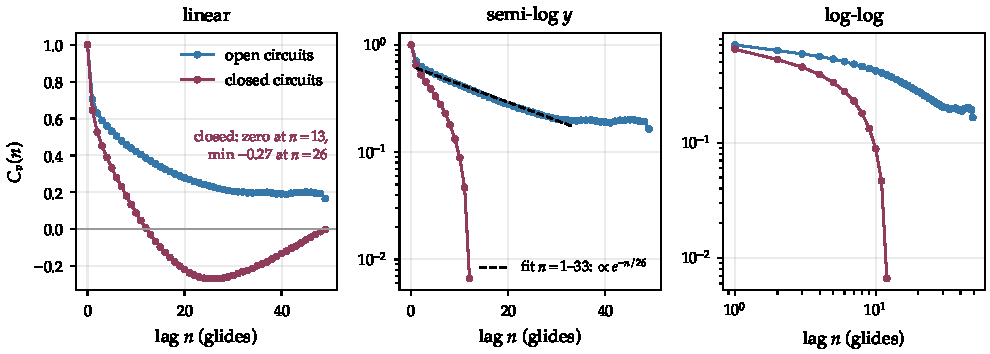
\includegraphics[width=146mm]{assets/glide-autocorrelation-para.pdf}};
 % Two take-home messages, one per line.
 \fill[pisablight!33](7,73.2)rectangle(153,83.6);
 \node[anchor=west,inner sep=0pt,text width=142mm,align=flush left,text=pisablue,font=\bfseries\boldmath\fontsize{10}{12.6}\selectfont]at(10,78.4){Open vs closed: very different motion from the first lags.\\
  Open: $C_v\approx\GlideFitA\,e^{-n/\GlideFitXi}$ up to $n=\GlideFitHi$: diffusive at long times?};
 \credit{Paragliders, fixed cohort: flights with at least \GlideCohortGlides\ glides in one segment (\GlideOpenFlights\ open, \GlideClosedFlights\ closed), each weighted equally.}
\speaker{First look at the data behind the model of the previous slide. Each Vilpellet glide (transition run) gets one mean velocity vector, $\mathbf v_k=\Delta\mathbf r_k/T_k$: the horizontal displacement vector from the start to the end of the glide, divided by its duration. Glides are numbered in time order inside a cleaned segment.\par\medskip
Fixed cohort: only flights with at least \GlideCohortGlides\ glides in one segment enter (\GlideOpenFlights\ open and \GlideClosedFlights\ closed circuits, paragliders), so every flight contributes to every lag up to $n=\GlideMaxLag$ and the population does not change with the lag. For each flight, $\mathbf v_k\cdot\mathbf v_{k+n}$ is averaged over all its pairs $n$ glides apart; these flight averages are then averaged with equal weight and divided by the mean squared glide speed. $C_v$ is not centred: a common route direction shows up as a positive value at long lags.\par\medskip
Open circuits: $C_v(1)=\GlideOpenOne$, slow monotone decay, still \GlideOpenLast\ at $n=\GlideMaxLag$. A straight line in semi-log $y$ over $n=\GlideFitLo$--$\GlideFitHi$ gives $C_v\approx\GlideFitA\,e^{-n/\GlideFitXi}$: a first hint of exponential memory loss, hence of diffusive motion at long times. Only a first check: the decay slows down with the lag and the curve flattens near \GlideOpenLast; a positive plateau would be a persistent route direction, i.e.\ a ballistic drift. Next check: remove each flight's mean velocity. Closed circuits: $C_v(1)=\GlideClosedOne$, zero at $n=\GlideClosedZero$, minimum \GlideClosedMin\ at $n=\GlideClosedMinLag$, back to about zero at $n=\GlideMaxLag$: to close the circuit the pilot must fly back.\par\medskip
Consequence for the model: the two circuit types already differ after the first glides, as they do for $H$, so they should be treated as two separate classes of motion. Angular diffusion alone cannot produce either the persistent direction of open circuits or the anticorrelation of closed ones; treat the two separately or remove each flight's mean direction. No error bars yet.}
\finishslide\end{frame}

% 9 ---------------------------------------------------------------------
\begin{frame}[plain]
\startslide{sFive}{5}{Solo vs group flights}{30 Nov -- 23 Dec \textperiodcentered{} 3 weeks}
 % Two scenes in plan view: same start but different paths; flying together.
 \foreach \x/\t in {7/{Same take-off cell, same 20 min},49/{Flying together}}{
  \card{\x}{16}{39}{50}{sFive}
  \smalltxt[text=sFive!75!black,font=\bfseries\fontsize{9}{10.5}\selectfont,align=center]{\x+1}{18}{37}{\t}}
 \begin{scope}[shift={(26.5,28.5)},scale=1.12,shift={(-25.75,-25)}]
 % Left: four flights leave the same cell within 20 minutes; two follow similar routes, two do not.
 \draw[muted,dashed,line width=.6pt](10.5,47)rectangle(17.5,54);
 \draw[muted,line width=.5pt](20.6,55.4)circle(1.5);\draw[muted,line width=.5pt](20.6,54.4)--(20.6,55.4)--(21.4,55.8);
 \node[anchor=west,inner sep=0pt,text=muted,font=\fontsize{6.5}{7.5}\selectfont]at(22.6,55.4){20 min};
 \begin{scope}[line width=.8pt]
  \draw[flA](13,50)to[bend left=10](19,41);\loops{19}{41}{flA}{1.1}{2}\draw[flA](20,41)to[bend right=8](28,34);\loops{28}{34}{flA}{1.1}{2}\draw[flA](29,34)--(38,27.5);
  \draw[flB](15,49)to[bend left=6](21.5,42.5);\loops{21.5}{42.5}{flB}{1.1}{2}\draw[flB](22.5,42.5)to[bend left=5](32,39.5);\loops{32}{39.5}{flB}{1.1}{2}\draw[flB](33,39.5)--(41,37.5);
  \draw[flC](12.5,48.5)to[bend right=10](11.5,38);\loops{11.5}{38}{flC}{1.1}{2}\draw[flC](12.5,38)--(13,30);\loops{13}{30}{flC}{1.1}{1.5}\draw[flC](13.75,30)--(16,25.5);
  \draw[flD](16,51.5)to[bend right=8](27,51);\loops{27}{51}{flD}{1.1}{2}\draw[flD](28,51)--(40,47);
 \end{scope}
 \foreach \p in {(13,50),(15,49),(12.5,48.5),(16,51.5)}{\fill[pisablue]\p circle(.45);}
 \end{scope}
 \begin{scope}[shift={(68.5,28.5)},scale=1.12,shift={(-66,-25)}]
 % Right: three flights leave a common cell within 20 minutes and follow the same thermals.
 \draw[muted,dashed,line width=.6pt](49,49.5)rectangle(57,55);
 \draw[muted,line width=.5pt](61,55.4)circle(1.5);\draw[muted,line width=.5pt](61,54.4)--(61,55.4)--(61.8,55.8);
 \node[anchor=west,inner sep=0pt,text=muted,font=\fontsize{6.5}{7.5}\selectfont]at(63,55.4){20 min};
 \foreach \p in {(56,43),(66,35),(77,28)}{\fill[rising!16]\p circle(2.8);}
 \begin{scope}[line width=.8pt]
  \draw[flA](49.5,53)to[bend left=14](55.2,43.6);\loops{55.2}{43.6}{flA}{1.1}{2}\draw[flA](56.2,43.6)to[bend left=12](65.2,35.6);\loops{65.2}{35.6}{flA}{1.1}{2}\draw[flA](66.2,35.6)to[bend left=8](76.4,28.6);\loops{76.4}{28.6}{flA}{1.1}{2}\draw[flA](77.4,28.6)--(81.5,25);
  \draw[flB](52.5,52.5)to[bend left=2](56.2,42.8);\loops{56.2}{42.8}{flB}{1.3}{1.5}\draw[flB](56.95,42.8)to(66.4,34.6);\loops{66.4}{34.6}{flB}{1.2}{2}\draw[flB](67.4,34.6)to[bend right=4](72.5,31.6);
  \draw[flC](55.5,53.5)to[bend right=14](56.6,44.4);\loops{56.6}{44.4}{flC}{1}{2.5}\draw[flC](57.85,44.4)to[bend right=14](65.8,36.6);\loops{65.8}{36.6}{flC}{1.1}{1}
 \end{scope}
 \foreach \p in {(49.5,53),(52.5,52.5),(55.5,53.5)}{\fill[pisablue]\p circle(.45);}
 \foreach \p/\c in {(81.5,25)/flA,(72.5,31.6)/flB,(66.3,36.6)/flC}{\fill[\c,draw=white,line width=.4pt]\p circle(.9);}
 \end{scope}
 \smalltxt[text=muted,font=\fontsize{8}{9.5}\selectfont,align=center]{7}{67.3}{39}{same start, different paths}
 \smalltxt[text=muted,font=\fontsize{8}{9.5}\selectfont,align=center]{49}{67.3}{39}{same thermals}
 % First a definition, then the analysis.
 \card{92}{16}{61}{22}{sFive}
 \badge{sFive}{97.5,22}{1}
 \txt[text=sFive!75!black,font=\bfseries\fontsize{10.5}{12.5}\selectfont]{103}{19}{48}{An operational definition}
 \smalltxt[font=\fontsize{9}{11}\selectfont]{103}{25.6}{48}{Same take-off cell +\\same departure window\\\textbf{does not imply group flight}}
 \arrowto{sFive}{122.5,38.5}{122.5,43.5}{}
 \card{92}{44}{61}{22}{sFive}
 \badge{sFive}{97.5,50}{2}
 \txt[text=sFive!75!black,font=\bfseries\fontsize{10.5}{12.5}\selectfont]{103}{47}{48}{Then the analysis}
 \smalltxt[font=\fontsize{9}{11}\selectfont]{103}{53.6}{48}{solo vs group: where they agree and where they differ}
 % Then compare with the toolbox.
 \node[anchor=west,inner sep=0pt,text=pisablue,font=\bfseries\fontsize{9.5}{11}\selectfont](c0)at(7,77){Then compare with step 3:};
 \foreach \l [count=\i, remember=\i as \j (initially 0)] in {MSD and $H$,scaling,memory,phase durations}{
  \node[anchor=west,inner xsep=1.4mm,inner ysep=1.1mm,rounded corners=1.2mm,fill=sThree!12,draw=sThree!60,line width=.5pt,font=\fontsize{8}{9.5}\selectfont,text height=1.6ex,text depth=.4ex](c\i)at([xshift=2.5mm]c\j.east){\l};}
\speaker{Two steps. First, an operational definition of group flight: both sketches show departures from a common cell within the same 20-minute window, but only the right-hand group follows the same thermals. A common departure window alone does not establish group flight. The current viewer lists only candidates: departures from the same 5 km cell within a 30-minute window. The first task is to find the definition that groups the real group flights, separating them from flights that simply share a site, a day or a route; weather and common routes alone can create correlated motion.\par\medskip
Second, the comparison: once the labels are reliable, apply the toolbox of step 3 to solo and group flights (MSD and $H$, scaling, memory, phase durations) to see where they are similar and where they differ. Uncertainty must be computed at the level of site and day or of the group, since group members are not independent.}
\finishslide\end{frame}

% 10 --------------------------------------------------------------------
\begin{frame}[plain]
\startslide{sSix}{6}{Optimal path: an exploratory direction}{4 Jan -- 7 Feb \textperiodcentered{} 5 weeks}
 \node[anchor=north west,inner sep=0pt]at(7,18){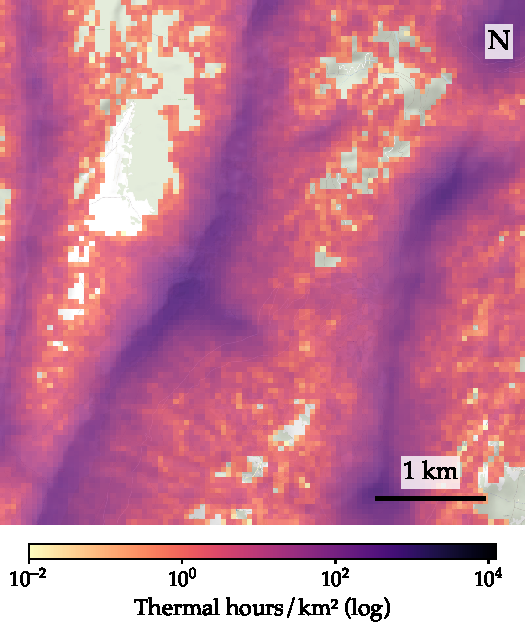
\includegraphics[width=48mm]{assets/thermal-density-chartreuse.pdf}};
 \smalltxt[text=muted,font=\fontsize{7}{8.5}\selectfont]{7}{76.5}{48}{Chartreuse, $5\times5$\,km.\\All years pooled.}
 % The first step defines what distribution the climb data should estimate.
 \card{60}{18}{93}{18}{sSix}
 \badge[2.5]{sSix}{64.5,24}{\fontsize{7.5}{8}\selectfont 1}
 \txt[text=sSix!80!black,font=\bfseries\boldmath\fontsize{10.5}{12}\selectfont]{70}{20}{79}{Data on glider climb segments\\$\longrightarrow$ a thermal distribution $P(x,y)$}
 \smalltxt[font=\fontsize{9}{10.5}\selectfont]{70}{30}{79}{Several definitions, depending on the research question.}
 % From the empirical distributions to an optimal path.
 \foreach \n/\y/\h/\t in {
  2/38.5/10.5/{Updraft distribution $p(w\mid\mathrm{site})$\\$w$: vertical air velocity},
  3/66/10.5/{Optimal 2D path for each terrain type,\\using the thermal distributions from the data},
  4/79/7/{Compare optimal paths with recorded flights}}{
  \card{60}{\y}{93}{\h}{sSix}
  \badge[2.5]{sSix}{64.5,\y+\h/2}{\fontsize{7.5}{8}\selectfont\n}
  \node[anchor=west,inner sep=0pt,text width=79mm,align=flush left,font=\fontsize{10}{11.5}\selectfont]at(70,\y+\h/2){\t};}
 % Compare both distributions between terrain types and between sites.
 \draw[sSix!65,line width=.8pt](60,51)--(60,63.5);
 \smalltxt[font=\fontsize{9.3}{11.3}\selectfont]{64}{51}{89}{%
  \textcolor{sSix!80!black}{\textbf{How do both distributions change?}}\\
  between terrain classes: mountains, hills, plains\\
  within one class: from one mountain (or plain) to another}
 \foreach \y in {36,63.5,76.5}{\arrowto{sSix}{106.5,\y}{106.5,\y+2.5}{}}
\speaker{Compute an optimal trajectory from empirical thermal distributions and compare it with recorded flights. Almgren and Tourin (2015) use Hamilton--Jacobi--Bellman equations; I have not studied the paper yet. A 2D extension is exploratory.\par\medskip
Steps 1 and 2 estimate $P(x,y)$ from glider climb segments and the updraft distribution $p(w\mid\mathrm{site})$. Define what $P(x,y)$ counts or weights, and its normalisation, according to the research question. The map shows cumulative climb time per area, not encounter probability. Here $w$ is vertical air velocity; observed climb rate is $\dot z=w-s_{\mathrm{sink}}$, so inferring $w$ requires a sink-rate model.\par\medskip
Compare both distributions across mountains, hills and plains, then across sites within each category. Test whether sites are compatible with a common distribution: a shared law is a hypothesis. Comparing spatial distributions also requires a meaningful common coordinate representation.\par\medskip
Step 3 uses these empirical distributions in a 2D control problem depending on terrain category. A shared distribution may provide a category-level model if supported by the data; otherwise retain site differences. The loss function and formulation remain to be defined. Step 4 compares optimal and recorded paths.\par\medskip
Sources: R.\ Almgren and A.\ Tourin, Optim.\ Control Appl.\ Meth.\ (2015), \href{https://doi.org/10.1002/oca.2122}{doi:10.1002/oca.2122}. Map: viewer Thermal density, Vilpellet, paragliders and hang gliders, all dates and heights; 50 m pixels, hours/km$^2$, fixed logarithmic scale. Background: IGN/G\'eoplateforme, Plan IGN.}
\finishslide\end{frame}

% 11 --------------------------------------------------------------------
\begin{frame}[plain]
\startslide{sTool}{}{The graphical tool: today and next}{in parallel}
 % Today.
 \card{7}{16}{146}{18}{muted}
 \begin{scope}[shift={(11,18)},scale=.38]
  \fill[white,draw=sTool,line width=1pt,rounded corners=1.2mm](0,0)rectangle(46,34);
  \fill[sTool,rounded corners=1.2mm](0,0)rectangle(46,4.5);\fill[sTool](0,2.5)rectangle(46,4.5);
  \fill[pisablight!40](2,6.5)rectangle(10,32);
  \begin{scope}\clip(12,6.5)rectangle(44,32);\fill[climb!6](12,6.5)rectangle(44,32);
   \foreach \r in {4,7,10,13}{\draw[muted!35,line width=.4pt](30,21)ellipse({1.6*\r} and \r);}\end{scope}
  \draw[glide,line width=1pt](14,29)..controls(18,26)and(21,25)..(24,22);
  \draw[climb,line width=.9pt,domain=0:1080,samples=150](24.5,21.5)plot({24.5+.003*\x+2.4*cos(\x)},{21.5-.007*\x+.9*sin(\x)});
  \draw[glide,line width=1pt](30,14)..controls(34,13)and(38,11)..(42,9);
 \end{scope}
 \txt[text=muted!80!black,font=\bfseries\fontsize{11}{13}\selectfont]{33}{18.6}{20}{Today}
 \smalltxt[font=\fontsize{9.5}{11.5}\selectfont]{51}{19.2}{44}{Works, but \textbf{not reviewed or tested}}
 \smalltxt[font=\fontsize{9.5}{11.5}\selectfont]{103}{19.2}{48}{Mixed with the analysis code, so it \textbf{runs only on my Mac}}
 \draw[muted!50,line width=.5pt](98,19)--(98,31);
 % Two paths.
 \card{7}{39}{70}{31}{sFive}
 \txt[text=sFive!75!black,font=\bfseries\fontsize{11}{13}\selectfont]{11}{41.6}{64}{Short term: today's viewer}
 \smalltxt[font=\fontsize{9.5}{11.5}\selectfont]{11}{49.5}{63}{%
  \bulitem{own repository, runs on any PC}
  \bulitem{no new work on it}}
 \smalltxt[text=sFive!75!black,font=\bfseries\fontsize{9.5}{11}\selectfont]{11}{63.5}{63}{Usable soon, still unreviewed}
 \card{83}{39}{70}{31}{sTool}
 \txt[text=sTool!80!black,font=\bfseries\fontsize{11}{13}\selectfont]{87}{41.6}{64}{In parallel: a clean viewer}
 \smalltxt[font=\fontsize{9.5}{11.5}\selectfont]{87}{49.5}{63}{%
  \bulitem{reviewed, one-way imports, any PC}
  \bulitem{all new features go here}}
 \smalltxt[text=sTool!80!black,font=\bfseries\fontsize{9.5}{11}\selectfont]{87}{63.5}{63}{Trustworthy, but it takes longer}
 \bottomline{Make today's viewer usable by everyone, but invest the time only in the clean viewer}
\speaker{The viewer was built with Claude, on top of analysis code that has not been reviewed. It works, and it has been very useful, but it has not been properly reviewed and tested, so we cannot be sure that everything it shows is computed as it should be. Its code is mixed with the analysis code of the repository that holds everything written so far, with imports in both directions: this is the main reason why today it hardly runs on any computer other than mine.\par\medskip
Two things can be done, with different roles. In the short term, move today's viewer, unreviewed, to a separate repository and spend some time making it run on other computers. It is a temporary solution, but it lets everyone use the current viewer soon, knowing it is not reviewed; it should not do much harm. In parallel, and over a longer time, build a clean viewer: reviewed code, which imports the tools of the clean analysis repository in one direction only, designed from the start to run on any PC and to be easy to install and use. Both take time, which is why the tool runs as a parallel track for the whole internship. Because today's viewer is so entangled with the analysis code, it makes no sense to keep improving it: once it runs everywhere, it stays as it is. New features and fixes go into the clean viewer, so that the time is spent on code meant to be used by everyone, reviewed and kept in the long run.}
\finishslide\end{frame}

% 12 --------------------------------------------------------------------
\begin{frame}[plain]
\startslide{pisablue}{}{Organising the code}{repositories over time}
 % Repositories over time (schematic, not to scale).
 \foreach \x/\l in {44/today,62/soon,80/{12 Oct \textperiodcentered{} step 2}}{
  \draw[muted!50,dashed,line width=.5pt](\x,21.5)--(\x,65.5);
  \node[anchor=base,inner sep=0pt,text=muted,font=\bfseries\fontsize{7.8}{9}\selectfont]at(\x,20){\l};}
 \node[anchor=base east,inner sep=0pt,text=muted,font=\bfseries\fontsize{7.8}{9}\selectfont]at(153,20){Feb 2027 $\rightarrow$};
 % One lane per repository: name on the left, life span as a bar.
 \foreach \y/\c/\n/\d in {26/sFive/Exploration/{the repository of today},37/sTwo/Analysis (new)/{definitive analyses},48/sTool/Viewer (clean)/{see previous slide},59/sTool/Viewer (today's)/{see previous slide}}{
  \node[anchor=west,inner sep=0pt,text=\c!80!black,font=\bfseries\fontsize{9}{10.5}\selectfont]at(7,\y+1.4){\n};
  \node[anchor=west,inner sep=0pt,text=muted,font=\fontsize{6.8}{8}\selectfont]at(7,\y+4.6){\d};}
 \fill[sFive!22,draw=sFive,line width=.6pt,rounded corners=.8mm](44,26)rectangle(153,30.6);
 \node[anchor=west,inner sep=0pt,text=sFive!70!black,font=\fontsize{7.5}{9}\selectfont]at(46,28.3){all the code so far, messy and unreviewed; later only quick tests and ``vibe coding''};
 \fill[sTwo!18,draw=sTwo,line width=1.2pt,rounded corners=.8mm](80,37)rectangle(153,41.6);
 \node[anchor=west,inner sep=0pt,text=sTwo!80!black,font=\bfseries\fontsize{7.5}{9}\selectfont]at(82,39.3){clean, reviewed and tested code for steps 1--6};
 \shade[left color=white,right color=sTool!18,rounded corners=.8mm](98,48)rectangle(118,52.6);
 \fill[sTool!18,rounded corners=.8mm](116,48)rectangle(153,52.6);
 \draw[sTool,line width=.6pt,rounded corners=.8mm,dash pattern=on 1.5pt off 1pt](98,48)--(116,48)(98,52.6)--(116,52.6);
 \draw[sTool,line width=.6pt,rounded corners=.8mm](116,48)--(153,48)--(153,52.6)--(116,52.6);
 \node[anchor=west,inner sep=0pt,text=sTool!80!black,font=\fontsize{7.5}{9}\selectfont]at(100,50.3){built step by step; one-way imports};
 \fill[sTool!10,draw=sTool!70,line width=.6pt,dashed,rounded corners=.8mm](62,59)rectangle(153,63.6);
 \node[anchor=west,inner sep=0pt,text=sTool!80!black,font=\fontsize{7.5}{9}\selectfont]at(64,61.3){moved as it is, made to run on any PC; no new work on it};
 % Where each repository comes from.
 \draw[-{Latex[length=1.8mm]},sTool,line width=.9pt](62,30.8)--(62,58.8);
 \node[anchor=west,inner sep=0pt,text=muted,font=\fontsize{6.8}{8}\selectfont]at(63.2,46){split off};
 \draw[-{Latex[length=1.8mm]},sFive,line width=.9pt,dashed](80,30.8)--(80,36.8);
 \node[anchor=west,inner sep=0pt,text=muted,font=\fontsize{6.8}{8}\selectfont]at(81.2,33.9){ideas, rewritten and reviewed};
 \draw[-{Latex[length=1.8mm]},sTwo,line width=.9pt](108,41.8)--(108,47.8);
 \node[anchor=west,inner sep=0pt,text=muted,font=\fontsize{6.8}{8}\selectfont]at(109.2,44.9){one-way import};
 \bottomline{Explore fast in one place; build the internship results only on reviewed code}
\speaker{Today there is one repository with everything: download, cleaning, experiments, analyses and the viewer. It was written with Claude to explore as much as possible, as fast as possible, and much of it has never been reviewed. That is fine for exploring, not for the results of the internship.\par\medskip
The plan over time. Soon, today's viewer is split off, as it is, into its own repository and made to run on any PC (previous slide); no new work goes into it. From 12 October, with step 2, a new repository with clean, reviewed and tested code holds the definitive analyses of each step. In parallel, step by step, a clean viewer is built on top of it, importing the analysis tools in one direction only (previous slide). The current repository stays for exploration, quick tests and ``vibe coding''; ideas that work there are rewritten and reviewed in the clean one, never copied over as they are. Reviewing takes much more time than writing, but it is the only way to be sure that everything works as expected.}
\finishslide\end{frame}



\end{document}
